\documentclass[conference]{IEEEtran}
\IEEEoverridecommandlockouts

\usepackage{cite}
\usepackage{amsmath,amssymb,amsfonts}
\usepackage{algorithmic}
\usepackage{algorithm}
\usepackage{graphicx}
\usepackage{booktabs}
\usepackage{textcomp}

% Every number that appears in the prose (\headline, split sizes, seeds,
% crossovers) is generated by src/make_tables.py from results/tables/.
% AUTO-GENERATED by src/make_tables.py -- do not edit by hand.
\newcommand{\headline}{58.5\%}
\newcommand{\nTasks}{10,000}
\newcommand{\nTrainTasks}{8,012}
\newcommand{\nTestTasks}{1,988}
\newcommand{\trainPercent}{80}
\newcommand{\seedValue}{42}
\newcommand{\quantumValue}{4}
\newcommand{\crossoverUniform}{1.5}
\newcommand{\crossoverLognormal}{2}
\newcommand{\sigmaLinear}{2.21}
\newcommand{\sigmaGBM}{1.72}
\newcommand{\wFCFS}{167}
\newcommand{\wRR}{11.5}
\newcommand{\wExpAvg}{63.2}
\newcommand{\wLinear}{39.4}
\newcommand{\wGBM}{29.6}
\newcommand{\wOracle}{5.78}
\newcommand{\ratioExpAvgOracle}{10.9}
\newcommand{\ratioExpAvgRR}{5.48}
\newcommand{\ratioGBMRR}{2.56}
\newcommand{\ratioLinearGBM}{1.33}
\newcommand{\maeSpreadPct}{2.92}
\newcommand{\underExpAvg}{18.5}
\newcommand{\underLinear}{48.3}
\newcommand{\underGBM}{28.1}
\newcommand{\wNoiseAtSigmaGBM}{10.2}
\newcommand{\ratioGBMNoise}{2.9}
\newcommand{\longTaskThreshold}{10,000}
\newcommand{\nLongTest}{11}
\newcommand{\longGBMMin}{10.6}
\newcommand{\longGBMMax}{264}
\newcommand{\maxGBMPred}{493}
\newcommand{\maxActual}{104,558}
\newcommand{\medianActual}{6}
\newcommand{\spearmanGBM}{0.66}
\newcommand{\spearmanLinear}{0.09}
\newcommand{\spearmanExpAvg}{0.14}
\newcommand{\meanExpAvgPred}{202}
\newcommand{\testWindow}{75}


\def\BibTeX{{\rm B\kern-.05em{\sc i\kern-.025em b}\kern-.08em
    T\kern-.1667em\lower.7ex\hbox{E}\kern-.125emX}}

\begin{document}

\title{Learned Burst-Time Prediction for Shortest-Remaining-Time-First CPU Scheduling:\\
An Empirical Study on a Production Cluster Trace}

% TODO(author): confirm school, campus and whether a personal e-mail address is
% wanted in the published version.
\author{\IEEEauthorblockN{Dheerajkumar Sasikumar}
\IEEEauthorblockA{\textit{B.Tech.\ Artificial Intelligence and Machine Learning} \\
\textit{Vellore Institute of Technology}\\
dheerajsm2007@gmail.com}}

\maketitle

\begin{abstract}
Shortest-remaining-time-first (SRTF) scheduling minimises mean waiting time on
a single processor only when the service demand of every task is known in
advance; operating systems approximate that demand by exponential averaging of
past bursts. This paper asks how much of the gap between exponential-averaging
SRTF and clairvoyant (oracle) SRTF can be recovered by replacing the estimator
with a supervised model trained on features observable when a task arrives.
Using the first \nTasks{} tasks of the Alibaba cluster-trace-v2018 batch
workload, a leakage-safe feature set was constructed with a causal event
timeline, six predictors (exponential averaging, last-two averaging, a median
baseline, linear regression, gradient-boosted trees and an oracle) were
evaluated on a chronological split, and each was embedded in a discrete-event
single-CPU simulator alongside first-come-first-served and round-robin
baselines. The gradient-boosted predictor recovered \headline{} of the
waiting-time gap between exponential-averaging SRTF and oracle SRTF, yet no
prediction-driven scheduler outperformed round robin on this workload. A
sensitivity analysis with bounded-uniform and log-normal prediction noise
locates the error level at which SRTF loses its advantage over round robin and
shows that the errors of the fitted models are structured rather than random:
the gradient-boosted model waits about \ratioGBMNoise{} times longer than
random error of the same spread would imply, because it systematically
under-predicts the rare very long tasks. Mean absolute error does not
predict scheduling quality; rank agreement with the true runtime does. All
tables, figures and numbers are generated programmatically from the
experiment outputs.
\end{abstract}

\begin{IEEEkeywords}
CPU scheduling, shortest remaining time first, runtime prediction, machine
learning, cluster traces, leakage-safe evaluation
\end{IEEEkeywords}

\section{Introduction}
\label{sec:introduction}

\subsection{Motivation}
Shortest-remaining-time-first (SRTF), the preemptive form of
shortest-job-first, minimises mean waiting time on a single
processor~\cite{schrage_optimality_1968}. It is also taught as a policy that
cannot be implemented exactly, because the length of the next CPU burst is
unknown when the scheduling decision is made~\cite{silberschatz_os_2018}.
The textbook remedy is to estimate that length by exponential averaging of
previous bursts. Meanwhile, learned components have displaced hand-designed
heuristics elsewhere in computer systems, including index
structures~\cite{kraska_case_2018}, cache
replacement~\cite{vietri_driving_2018,rodriguez_learning_2021,shi_applying_2019,song_learning_2020}
and compiler optimisation~\cite{wang_machine_2018}. It is therefore natural
to ask whether a supervised model, trained only on information available
when a task arrives, is a better estimator for SRTF, and how much of SRTF's
theoretical advantage such an estimator actually delivers.

\subsection{The Size and Location of the Gap}
On the workload studied here, the room for a better estimator is large.
Oracle SRTF, which is given every task's true runtime, achieves a mean
waiting time of \wOracle{}\,h per task, while SRTF driven by exponential
averaging waits \wExpAvg{}\,h, a factor of \ratioExpAvgOracle{} worse
(Table~\ref{tab:schedulers}). The same table shows that round robin, which
uses no runtime estimate at all, waits \wRR{}\,h, which is \ratioExpAvgRR{}
times less than exponential-averaging SRTF. The question that matters to a
scheduler designer is therefore not whether machine learning can beat
exponential averaging. It is whether any predictor restricted to
arrival-time information can make SRTF competitive with a policy that needs
no prediction at all.

\subsection{Approach and Principal Findings}
This paper answers that question empirically on the first \nTasks{} tasks of
the Alibaba cluster-trace-v2018 batch
workload~\cite{cheng_characterizing_2018}. Six predictors, from exponential
averaging to gradient-boosted trees, are trained on leakage-safe features and
evaluated on a chronological split, and each one drives SRTF in a
discrete-event single-CPU simulator. The gradient-boosted predictor recovers
\headline{} of the waiting-time gap between exponential-averaging SRTF and
oracle SRTF, yet it still waits \ratioGBMRR{} times longer than round robin,
and no prediction-driven SRTF outperforms round robin.

This negative result is the principal finding, not a caveat. On this trace
the features available at arrival do not carry the information SRTF needs
most, namely which of the arriving tasks are the rare very long ones. A
two-model sensitivity analysis shows why the fitted models fall short of
what their aggregate error suggests: their errors are concentrated on
exactly those long tasks.

\subsection{Contributions}
\begin{enumerate}
  \item A leakage-safe feature pipeline and set of online baselines on a real
    production trace, with unit tests that fail if any task still running at
    another task's arrival contributes to that task's features or
    predictions.
  \item An end-to-end mapping from prediction error to scheduling outcome.
    The recovered fraction of the gap, (\ref{eq:recovery}), and rank
    agreement are reported next to conventional error metrics, and the
    results show that mean absolute error does not predict scheduling
    quality.
  \item A two-model sensitivity analysis, bounded uniform and log-normal,
    that locates the error level at which SRTF loses to round robin and
    shows that structured error costs far more waiting time than random
    error of the same spread.
  \item A reproducible artefact in which every table, figure and number in
    the text is generated from the experiment outputs.
\end{enumerate}

\subsection{Organisation}
Section~\ref{sec:related} reviews related work.
Section~\ref{sec:problem} formalises the scheduling and prediction problem,
Section~\ref{sec:method} describes the implementation and
Section~\ref{sec:setup} the experimental setup. Section~\ref{sec:results}
presents and interprets the results, Section~\ref{sec:threats} discusses
threats to validity and Section~\ref{sec:conclusion} concludes.

\section{Related Work}
\label{sec:related}

% VERIFY-CLAIM(author): the one-line characterisations of prior work below
% follow LITERATURE.md. Check each against the full text before submission,
% in particular what Helmy et al. and Effah et al. measured and how Tsafrir
% et al. correct predictions that a job outlives.

\subsection{Burst-Time Prediction for CPU Scheduling}
Predicting resource demand to inform scheduling predates machine learning.
Dinda~\cite{dinda_prediction_2002} built a real-time scheduling advisor on
predicted running times. The Network Weather Service line of work forecast
network performance and CPU availability from
time series~\cite{wolski_dynamically_1998,wolski_predicting_2000,yang_homeostatic_2003},
and Zhang et al.~\cite{zhang_predict_2008} predicted task running times in
grids from CPU-load predictions. Helmy et al.~\cite{helmy_machine_2015}
framed CPU-burst estimation as supervised learning, training
nearest-neighbour, support-vector, neural-network and decision-tree models on
16 process features from the GWA-T-4 grid trace. Jha and
Goyal~\cite{jha_cpu_2022} pursued the same goal, and Pourali et
al.~\cite{pourali_fuzzy_undated} used a fuzzy rather than a learned model.
Effah et al.~\cite{effah_predicting_2025} is the closest prior work to this
paper: it predicts burst times to drive SJF and SRTF, but on a synthetic
dataset modelled on GWA-T-4. Shafin and Ahmed~\cite{shafin_leakage_2026}
revisited the Helmy formulation with a strict pre-submission feature policy
and chronological baselines, and this paper adopts their leakage-safe
framing. The present work differs from this line in two respects. It uses a
real production trace under a chronological split, and it reports the
waiting time that prediction accuracy buys, not prediction accuracy alone.

\subsection{Runtime Prediction for HPC Backfilling}
The richest neighbouring literature concerns runtime estimates for
backfilling batch schedulers. User-requested runtimes are known to be poor
estimates~\cite{lee_are_2004,lee_user_2006}, and Chiang et
al.~\cite{chiang_impact_2002} showed that more accurate requested runtimes
improve production scheduling performance, which is the premise behind the
recovery metric of this paper. Tsafrir et al.~\cite{tsafrir_backfilling_2007}
replaced user estimates with system-generated predictions from each user's
last two jobs, the origin of the Last2 baseline used here, and Gaussier et
al.~\cite{gaussier_improving_2015} used online regression for the same
purpose. Later work applied ensembles, transformers and automata-based deep
models~\cite{chen_runtime_2020,chen_job_2023,cheon_ared_2023}, predicted from
system logs~\cite{chen_predicting_2013}, and predicted other job
resources~\cite{tanash_improving_2019}. Because an under-estimate can get a
job killed at its walltime limit, a separate strand targets under-estimation
directly, through Tobit adjustment~\cite{fan_tobit_undated}, dedicated
predictors~\cite{unknown_machine_2017}, soft
walltimes~\cite{chlumsky_improving_2022} and uncertainty-aware quantile
prediction~\cite{unknown_uarp_2026}. TARE~\cite{xiao_tare_2026} argues that
mean-based metrics hide tail behaviour, which is why this paper reports the
under-prediction rate separately.

Single-CPU SRTF is a harsher consumer of predictions than backfilling.
Tsafrir et al. correct a prediction once a job outlives
it~\cite{tsafrir_backfilling_2007}, whereas the prediction-driven SRTF of
(\ref{eq:srtf-pred}) fixes the estimate at arrival and never revises it. An
under-predicted long task is therefore dispatched ahead of many short ones
and, once its predicted remaining time is exhausted, cannot be preempted.

\subsection{Learned Scheduling Policies}
A different line of work learns the scheduling policy itself with
reinforcement learning. DeepRM~\cite{mao_resource_2016} introduced the
approach for multi-resource cluster scheduling, and later variants refined
its state and action design~\cite{ye_new_undated,unknown_data_2020,domeniconi_cush_undated,cunha_impact_undated}.
Decima~\cite{mao_learning_2019} learned schedules for data-processing
clusters and reported large reductions in job completion time over
hand-tuned heuristics, and RLScheduler~\cite{zhang_rlscheduler_2020} applied
the approach to HPC batch scheduling. This paper deliberately does not learn
the policy. It keeps SRTF, which is optimal given true runtimes, and learns
only its input. The oracle then gives a known ceiling, and the part of the
gap that is due to the predictor can be measured directly, which an
end-to-end learned policy does not provide.

\subsection{Cluster Traces}
Public production traces underpin this line of research. The Google
traces~\cite{reiss_google_2011,chen_analysis_2010,reiss_heterogeneity_2012,liu_characterizing_2012}
document the Borg cluster manager's workload~\cite{verma_large_2015}. The
Alibaba traces capture co-located online services and batch
jobs~\cite{lu_imbalance_2017,cheng_characterizing_2018,cheng_analyzing_2018,liu_elasticity_2018,unknown_characterizing_2020}.
This study uses the batch-task table of the 2018 Alibaba release.

\section{Problem Formulation}
\label{sec:problem}

\subsection{Scheduling Model}
A single processor serves a finite set of $n$ tasks. Task $i$ becomes runnable
at its arrival time $a_i$ and requires $t_i$ units of processor time, its
\emph{runtime}. The scheduler may preempt the running task at any decision
point; preemption cost is not modelled. Let $S_i$ denote the instant at which
task $i$ first receives the processor and $C_i$ its completion instant. The
per-task metrics are the waiting time $W_i = C_i - a_i - t_i$, the turnaround
time $T_i = C_i - a_i$ and the response time $R_i = S_i - a_i$. The objective
is the mean waiting time $\bar{W} = \frac{1}{n}\sum_{i} W_i$.

\subsection{Shortest Remaining Time First}
Let $e_i(\tau)$ be the processor time that task $i$ has received by instant
$\tau$ and $\mathcal{R}(\tau)$ the set of runnable, incomplete tasks. At every
arrival and every completion, SRTF selects
\begin{equation}
  i^{*}(\tau) = \arg\min_{i \in \mathcal{R}(\tau)} \bigl( t_i - e_i(\tau) \bigr),
  \label{eq:srtf}
\end{equation}
the task with the least remaining service. When every $t_i$ is known at
$a_i$, this rule minimises $\bar{W}$ on a single
processor~\cite{schrage_optimality_1968}. No operating system knows $t_i$ in advance,
so (\ref{eq:srtf}) is a ceiling rather than an implementable policy; this
paper refers to it as \emph{oracle SRTF}.

\subsection{Prediction-Driven SRTF}
A prediction-driven scheduler replaces $t_i$ in (\ref{eq:srtf}) by an
estimate $\hat{t}_i = f(\mathbf{x}_i)$ computed once, when task $i$ arrives,
from a feature vector $\mathbf{x}_i$, and never revised afterwards:
\begin{equation}
  i^{*}(\tau) = \arg\min_{i \in \mathcal{R}(\tau)} \bigl( \hat{t}_i - e_i(\tau) \bigr).
  \label{eq:srtf-pred}
\end{equation}
The textbook estimator is exponential
averaging~\cite{silberschatz_os_2018}, which maintains a running estimate $\tau_n$ from the sequence of
observed runtimes $t_1, t_2, \ldots$ of the same source:
\begin{equation}
  \tau_{n+1} = \alpha\, t_n + (1 - \alpha)\, \tau_n, \qquad 0 \le \alpha \le 1 .
  \label{eq:expavg}
\end{equation}
In this work the source is the job identifier: one estimate is maintained per
job, updated at each completion of one of its tasks, and seeded with the
first observed runtime of that job. A task whose job has no completed history
is assigned the running mean of all completed runtimes.

\subsection{Prediction Target and Admissible Features}
The prediction target is the \emph{job-level runtime} recorded by the trace:
the wall-clock interval between the recorded start and end of a scheduled unit
of work (in the Alibaba trace, a \emph{task}, which is one stage of a job
executed by many instances). It is not the CPU burst between two I/O
operations that (\ref{eq:expavg}) was designed to estimate, and the paper
makes no claim to predict such bursts; the simulator treats this runtime as
the service demand $t_i$ in (\ref{eq:srtf}).

A feature is admissible only if its value is fixed at $a_i$. Historical
features of task $i$ are computed from
\begin{equation}
  \mathcal{H}_i = \{\, j : C_j < a_i \,\},
  \label{eq:causal}
\end{equation}
the set of tasks that completed \emph{strictly} before task $i$ arrived,
following the leakage-safe framing of Shafin and
Ahmed~\cite{shafin_leakage_2026}. A task that arrived earlier but is still
running at $a_i$ is excluded, and no train/test split is ever random.

\subsection{Evaluation Quantities}
Prediction quality is reported as mean absolute error, root mean squared
error, and the under-prediction rate, the fraction of tasks with
$\hat{t}_i < t_i$. The last is reported separately because aggregate error
metrics hide tail behaviour~\cite{xiao_tare_2026}, and because under- and
over-estimation of equal magnitude have very different consequences under
(\ref{eq:srtf-pred}): an under-estimated task's predicted remaining service
becomes negative as it runs and it can no longer be preempted. Because
(\ref{eq:srtf-pred}) consumes only the \emph{order} of the predictions,
the Spearman rank correlation $\rho_s$ between predicted and actual runtime
is reported as well.

Let $\bar{W}_{\mathrm{EA}}$, $\bar{W}_{\mathrm{GBM}}$ and
$\bar{W}_{\mathrm{OR}}$ denote the mean waiting time of SRTF driven by
exponential averaging, by the gradient-boosted predictor and by the oracle.
The headline quantity is the fraction of the gap that the learned predictor
recovers,
\begin{equation}
  \mathrm{recovery} =
  \frac{\bar{W}_{\mathrm{EA}} - \bar{W}_{\mathrm{GBM}}}
       {\bar{W}_{\mathrm{EA}} - \bar{W}_{\mathrm{OR}}} \times 100\% .
  \label{eq:recovery}
\end{equation}

\section{Methodology}
\label{sec:method}

The study was implemented as a five-stage pipeline: trace preprocessing,
causal feature construction, predictor training, discrete-event simulation,
and experiment orchestration. Each stage is described as implemented.

\subsection{Trace Preprocessing}
The \texttt{batch\_task} table was read in chunks of 500\,000 rows so that
the raw file was never resident in memory. Rows with a missing start or end
timestamp, a non-positive runtime, or a status other than
\texttt{Terminated} were discarded, in that order. The runtime was defined as
$t_i = \mathrm{end\_time}_i - \mathrm{start\_time}_i$. The table records no
submission timestamp, so the arrival time was set to
$a_i = \mathrm{start\_time}_i$; the consequences of this proxy are discussed
in Section~\ref{sec:threats}. The first $N$ tasks in ascending order of
(arrival time, job name, task name) were retained by maintaining a bounded
buffer of the earliest candidates across chunks. No random sampling was
performed, because the chronological split of Section~\ref{sec:setup}
depends on this ordering.

\subsection{Causal Feature Construction}
Historical features were computed in a single pass over a merged timeline of
$2N$ events, one arrival and one completion per task, sorted by time with
arrivals ordered before completions at equal timestamps so that
(\ref{eq:causal}) holds with strict inequality. An arrival event reads the
current state and fixes the task's features; a completion event appends the
task's runtime to its job's history and to a global running sum. Three
historical features result: \texttt{previous\_runtime}, the most recently
completed same-job runtime; \texttt{rolling\_mean\_3}, the mean of up to the
three most recently completed same-job runtimes; and \texttt{has\_history}, a
flag that is false when the job has no completed task yet. When the flag is
false both numeric features take the running mean of all completed runtimes;
when no task at all has completed they are undefined, and such rows were
excluded from the fitting of the regression models. Direct features were
taken from the task's own record or derived from $a_i$ alone. A unit test
asserts that a same-job task which arrived earlier but completes after $a_i$
does not contribute, and that the same test fails under a conventional
grouped shift over the arrival-sorted table.

\subsection{Predictors}
Six predictors share the interface $\mathrm{fit}(X_{\mathrm{train}},
y_{\mathrm{train}})$, $\mathrm{predict}(X)$.
\begin{itemize}
  \item \emph{Exponential averaging} implements (\ref{eq:expavg}) per job.
  \item \emph{Last2} predicts the mean of the two most recently completed
    same-job runtimes and falls back to the running global mean, following
    Tsafrir et al.~\cite{tsafrir_backfilling_2007}.
  \item \emph{Median} predicts the training-set median runtime for every
    task; it is the constant reference that any learned model must beat.
  \item \emph{Linear regression} is ordinary least squares on
    $\log(1 + t_i)$; the right-skewed inputs \texttt{n\_instances},
    \texttt{previous\_runtime} and \texttt{rolling\_mean\_3} are transformed
    by $\log(1 + x)$ and all inputs are standardised.
  \item \emph{Gradient boosting} is XGBoost~\cite{chen_xgboost_2016} on
    $\log(1 + t_i)$ with the configuration of Section~\ref{sec:setup}.
  \item \emph{Oracle} returns $t_i$ itself and defines the ceiling.
\end{itemize}
The logarithmic target was adopted because the runtime spans five orders of
magnitude and, in preliminary runs, squared-error regression on the raw
scale produced negative predictions for ordinary tasks. Predictions of
both regression models are mapped back with $\exp(\cdot) - 1$ and floored at
1\,s, the smallest runtime in the data. Exponential averaging and Last2 are
sequential estimators. $\mathrm{fit}$ stores the training events, and
$\mathrm{predict}$ walks one merged timeline of training and test arrivals
and completions from an empty state, as an online scheduler would. Each
completion updates the state only when it occurs, and each test prediction
is fixed at the task's arrival. A training task still running when a test
task arrives has therefore not yet been observed, and a unit test asserts
this across the train/test boundary.

\subsection{Discrete-Event Simulator}
A single-CPU simulator was written with one event loop per policy:
first-come-first-served (non-preemptive), round robin with a fixed quantum,
and predictor-driven SRTF. Algorithm~\ref{alg:srtf} gives the SRTF loop as
implemented. Predictions are obtained once for the whole task set by a single
call to the predictor and thereafter treated as constants. The loop tracks,
for the running task $r$, both the true remaining service $\rho_r$, which
determines when the task actually finishes, and the predicted remaining
service $\hat{t}_r - e_r$, which alone determines scheduling decisions.
Re-evaluation occurs at every arrival and every completion, and a slice runs
until the earlier of the running task's true completion and the next
arrival. A context switch is counted whenever the task starting a slice
differs from the task that ran in the preceding slice; the first slice is not
counted. When the predictor is the oracle, $\hat{t}_i = t_i$ and
Algorithm~\ref{alg:srtf} reduces to (\ref{eq:srtf}); a unit test asserts
per-task equality of first-dispatch, completion, waiting, turnaround and
response times between this configuration and an independently written
classical SRTF on a hand-worked four-process example and on five randomised
instances.

\begin{algorithm}[t]
\caption{Predictor-driven SRTF on a single CPU (as implemented)}
\label{alg:srtf}
\begin{algorithmic}[1]
\REQUIRE tasks $(a_i, t_i)$ sorted by $(a_i, \text{id})$; predictions $\hat{t}_i = f(\mathbf{x}_i)$ fixed at arrival
\STATE $\mathcal{R} \leftarrow \emptyset$; $r \leftarrow \bot$; $\tau \leftarrow a_1$; $e_i \leftarrow 0$ and $\rho_i \leftarrow t_i$ for all $i$
\WHILE{some task is incomplete}
  \STATE admit every unadmitted $i$ with $a_i \le \tau$ into $\mathcal{R}$
  \IF{$\mathcal{R} = \emptyset$ and $r = \bot$}
    \STATE $\tau \leftarrow$ next arrival time; \textbf{continue}
  \ENDIF
  \STATE $c \leftarrow \arg\min_{i \in \mathcal{R} \cup \{r\}} \bigl(\hat{t}_i - e_i,\; a_i,\; i\bigr)$ \COMMENT{lexicographic}
  \IF{$c \ne r$}
    \STATE if $r \ne \bot$: return $r$ to $\mathcal{R}$
    \STATE remove $c$ from $\mathcal{R}$; record $S_c \leftarrow \tau$ on first dispatch; $r \leftarrow c$
  \ENDIF
  \STATE $\delta \leftarrow \min(\rho_r,\; a_{\mathrm{next}} - \tau)$
  \STATE $\tau \leftarrow \tau + \delta$; $\rho_r \leftarrow \rho_r - \delta$; $e_r \leftarrow e_r + \delta$
  \IF{$\rho_r = 0$}
    \STATE $C_r \leftarrow \tau$; $r \leftarrow \bot$
  \ENDIF
\ENDWHILE
\end{algorithmic}
\end{algorithm}

\subsection{Experiment Orchestration}
A driver script fits every predictor on the training split, runs the seven
schedulers over the test split, writes the comparison table, aborts if the
oracle-driven SRTF is not the minimum-waiting-time scheduler, runs the two
sensitivity sweeps, and computes (\ref{eq:recovery}). A second script
converts the result tables into the LaTeX tables and numeric macros of this
paper, so that no reported number is transcribed by hand.

\section{Experimental Setup}
\label{sec:setup}

\subsection{Trace and Task Set}
The workload is the \texttt{batch\_task} table of the Alibaba
cluster-trace-v2018, an eight-day trace of a production cluster of about
4\,000 machines running co-located online services and batch
jobs~\cite{cheng_characterizing_2018,unknown_characterizing_2020}. Each row
is one task with the fields task name, instance count, job name, task type,
status, start time, end time, planned CPU (100 per core) and normalised
planned memory. The first \nTasks{} tasks in arrival order that satisfied
the filters of Section~\ref{sec:method} were retained; they span
approximately the first 24 hours of the trace.

\subsection{Chronological Split}
The task set was split at \trainPercent\% in arrival order, giving
\nTrainTasks{} training and \nTestTasks{} test tasks. Because many tasks
share an identical arrival timestamp, the boundary was advanced to the next
distinct arrival time rather than cutting a tied cluster, and the run aborts
unless the latest training arrival strictly precedes the earliest test
arrival. No random or shuffled split was used anywhere in the pipeline.

\subsection{Features}
Table~\ref{tab:features} lists every model input with the reason it is
available when the task arrives. No other input was used.

\begin{table}[t]
  \caption{Model inputs and why each is known at task arrival.}
  \label{tab:features}
  \centering
  \begin{tabular}{lp{0.60\columnwidth}}
    \toprule
    Feature & Availability at arrival \\
    \midrule
    \texttt{requested\_cpu} & Planned CPU declared in the task's own submitted record (\texttt{plan\_cpu}). \\
    \texttt{requested\_mem} & Planned memory declared in the same record (\texttt{plan\_mem}). \\
    \texttt{n\_instances} & Instance count declared in the same record (\texttt{instance\_num}). \\
    \texttt{hour\_of\_day} & $\lfloor (a_i \bmod 86\,400) / 3\,600 \rfloor$, a function of $a_i$ alone. \\
    \texttt{day\_of\_week} & $\lfloor a_i / 86\,400 \rfloor \bmod 7$, a function of $a_i$ alone. \\
    \texttt{previous\_runtime} & Runtime of the latest same-job task in $\mathcal{H}_i$ of (\ref{eq:causal}); the global running mean if there is none. \\
    \texttt{rolling\_mean\_3} & Mean of up to three latest same-job runtimes in $\mathcal{H}_i$; same fallback. \\
    \texttt{has\_history} & Whether $\mathcal{H}_i$ contains a same-job task; a property of past completions only. \\
    \bottomrule
  \end{tabular}
\end{table}

\subsection{Predictor Configuration}
Gradient boosting used 300 trees of maximum depth 4, learning rate 0.05, row
and column subsampling of 0.8, minimum child weight 5, the squared-error
objective on the logarithmic target, and \texttt{random\_state} equal to the
seed below. This configuration was selected among four candidates on a
chronological validation split formed from the last 20\% of the training
set; the test set was not consulted. Linear regression used the
scikit-learn ordinary-least-squares solver~\cite{pedregosa_scikit_2011}
behind a standardisation step, without
regularisation. Exponential averaging used $\alpha = 0.5$ in
(\ref{eq:expavg}); Last2 used a window of two; the median baseline used the
median of the training runtimes. Both regression models and the median
baseline were fitted on the training rows for which the historical features
are defined; rows that arrived before any task had completed were dropped
from fitting only, and the run aborts if any such row appears in the test
split.

\subsection{Schedulers and Sensitivity Sweeps}
Seven schedulers were compared: first-come-first-served, round robin with a
quantum of \quantumValue{} simulated seconds, and SRTF driven by each of
exponential averaging, Last2, linear regression, gradient boosting and the
oracle. The sensitivity sweeps replace $\hat{t}_i$ by the true runtime
perturbed by a noise model and floored at 1\,s: bounded uniform,
$\hat{t}_i = t_i (1 + U(-\varepsilon, \varepsilon))$ with
$\varepsilon \in \{0, 0.1, 0.2, 0.3, 0.5, 0.75, 1, 1.5, 2, 3, 5\}$, and
log-normal, $\hat{t}_i = t_i \exp(\sigma Z)$ with $Z \sim \mathcal{N}(0, 1)$
and $\sigma \in \{0, 0.25, 0.5, 1, 1.5, 2, 3\}$. For each sweep the crossover
is the smallest level at which SRTF's mean waiting time exceeds that of
round robin, and the run aborts unless the zero-noise level reproduces
oracle SRTF exactly.

\subsection{Random Seeds, Software and Hardware}
A single declared seed, \seedValue{}, is used as the XGBoost
\texttt{random\_state} and as the base of the sweep generators, which use
$\seedValue{} + k$ (uniform) and $\seedValue{} + 100 + k$ (log-normal) for
the $k$-th level. Preprocessing, feature construction, ordinary least
squares and the simulator are deterministic. The software stack was
Python~3.13.14, NumPy~2.5.3, pandas~3.0.5, scikit-learn~1.9.1,
XGBoost~3.4.1 and Matplotlib~3.11.2, run as a single process on an Intel
Core Ultra~9 275HX (24 cores) with 15.5\,GB of memory under Windows~11.
Wall-clock cost of inference and simulation was not measured and is not
charged against the simulated scheduler.

\section{Results and Discussion}
\label{sec:results}

Table~\ref{tab:prediction} reports the prediction error of every predictor on
the test split, Table~\ref{tab:schedulers} the scheduling outcomes of the
seven schedulers, and Table~\ref{tab:sensitivity} the two sensitivity sweeps.
Fig.~\ref{fig:waiting} plots average waiting time by scheduler against the
oracle ceiling, Fig.~\ref{fig:sensitivity} plots both sweeps against the
round-robin reference, and Fig.~\ref{fig:scatter} plots the gradient-boosted
predictions against the actual runtimes. By (\ref{eq:recovery}), the
gradient-boosted predictor recovers \headline{} of the waiting-time gap
between exponential-averaging SRTF and oracle SRTF. The uniform sweep first
exceeds the round-robin waiting time at $\varepsilon = \crossoverUniform$ and
the log-normal sweep at $\sigma = \crossoverLognormal$; the empirical
standard deviation of $\log(\hat{t}_i / t_i)$ over the test split is
\sigmaGBM{} for gradient boosting and \sigmaLinear{} for linear regression.

\subsection{Prediction Error Does Not Predict Scheduling Quality}
The three regression-style predictors, the constant median, linear
regression and gradient boosting, are within \maeSpreadPct\% of one another
in mean absolute error, and their root mean squared errors are nearly
identical (Table~\ref{tab:prediction}). Both metrics are dominated by a
handful of very long tasks: the median test runtime is \medianActual{}\,s,
but the longest test task runs for \maxActual{}\,s. Exponential averaging
and Last2 are worse still. Almost every test task belongs to a job with no
completed task, so both fall back to the running mean of completed runtimes,
around \meanExpAvgPred{}\,s, for nearly every task.

The scheduling outcomes separate these predictors sharply. Linear regression
and gradient boosting differ by less than \maeSpreadPct\% in mean absolute
error, yet SRTF driven by linear regression waits \ratioLinearGBM{} times
longer (Table~\ref{tab:schedulers}). The difference lies in ordering. SRTF
uses only the order of the predictions, and the Spearman correlation with
actual runtime is \spearmanGBM{} for gradient boosting but only
\spearmanLinear{} for linear regression and \spearmanExpAvg{} for
exponential averaging. Mean absolute error rewards predicting the typical
task well; a scheduler needs the order of the tasks right, especially at the
long end. This is why the recovery percentage of (\ref{eq:recovery}), not
mean absolute error, is the quantity reported as the headline.

\subsection{Scheduling Outcomes}
Oracle SRTF has the lowest mean waiting time of all seven schedulers, as it
must, and first-come-first-served the highest. Replacing exponential
averaging with gradient boosting reduces SRTF's mean waiting time from
\wExpAvg{}\,h to \wGBM{}\,h, recovering \headline{} of the gap to the
oracle. Round robin, however, waits only \wRR{}\,h, and no prediction-driven
SRTF comes close to it. Round robin pays for this with two orders of
magnitude more context switches, and its response time is lower than that
of every other policy because every task receives a quantum soon after it
arrives.

Two properties of the test split shape these outcomes. First, every test
task arrives within a window of \testWindow{}\,s, while the backlog takes
far longer to drain, so the problem is close to ordering a single batch.
Second, for linear regression, gradient boosting and the oracle, the number
of context switches equals the number of tasks minus one, and waiting time
equals response time. No task was ever preempted once started, so SRTF
reduced to non-preemptive shortest-predicted-job-first over that batch.
Under these conditions the cost of a mistake is simple. A long task that is
predicted to be short runs to completion ahead of every task ranked behind
it.

Fig.~\ref{fig:scatter} shows exactly this failure. Gradient-boosted
predictions saturate: the largest prediction on the test split is
\maxGBMPred{}\,s. The \nLongTest{} test tasks that run longer than
\longTaskThreshold{}\,s receive predictions between \longGBMMin{}\,s and
\longGBMMax{}\,s, indistinguishable from those of ordinary tasks. Their
records at arrival do not tell them apart from typical tasks.

\subsection{Sensitivity to Prediction Error}
Table~\ref{tab:sensitivity} and Fig.~\ref{fig:sensitivity} report SRTF under
synthetic prediction error. Under bounded uniform noise SRTF is remarkably
robust: its waiting time rises only slowly up to $\varepsilon = 1$, then
exceeds round robin at $\varepsilon = \crossoverUniform$. The mechanism is
the floor at 1\,s. Once $\varepsilon > 1$ the factor $1 + U(-\varepsilon,
\varepsilon)$ can be non-positive, some long tasks are predicted at 1\,s,
and each of them blocks the processor. The waiting time at
$\varepsilon = 5$ is lower than at $\varepsilon = 3$ because each level is a
single random draw; which long tasks happen to be floored varies between
draws.

The log-normal model produces multiplicative errors of the kind a fitted
model makes, and SRTF degrades smoothly under it, crossing round robin at
$\sigma = \crossoverLognormal$. The empirical log-error spread of gradient
boosting, $\sigma = \sigmaGBM$, lies inside the region where SRTF still beats
round robin, and random log-normal error of that spread yields about
\wNoiseAtSigmaGBM{}\,h of waiting by linear interpolation of the sweep. The
fitted model's actual waiting time is \wGBM{}\,h, about \ratioGBMNoise{}
times higher. Linear regression's spread, $\sigma = \sigmaLinear$, lies
beyond the crossover.

The difference is structure. Random error of a given spread is equally
likely to over- or under-predict any task, whereas the fitted model's error
is correlated with runtime: it systematically under-predicts the long tasks
whose placement dominates mean waiting time. Structured error of a given
spread therefore hurts SRTF far more than random error of the same spread.
The practical consequence is that a deployment decision cannot be made from
an error budget alone; it also depends on how the error correlates with the
runtime itself.

\subsection{Under-Prediction and the Fixed Estimate}
Under (\ref{eq:srtf-pred}) an under-predicted task's predicted remaining
service reaches zero while it still has work left, after which no arrival
can preempt it. The under-prediction rate of Table~\ref{tab:prediction} is
\underGBM\% for gradient boosting, \underLinear\% for linear regression and
\underExpAvg\% for exponential averaging. A low rate is not sufficient on its
own: exponential averaging under-predicts least of the three, yet schedules
worst, because its near-constant predictions carry almost no ordering
information. What matters is whether the \emph{long} tasks are
under-predicted, and for gradient boosting they all are. The underlying
design flaw is the rule of predicting once and never revising. A deployed
predictor should increase its estimate once a task's elapsed service
exceeds it, as backfilling schedulers already
do~\cite{tsafrir_backfilling_2007}. This is the concrete engineering
recommendation of this study.

% AUTO-GENERATED by src/make_tables.py -- do not edit by hand.
\begin{table}[t]
  \caption{Prediction error on the chronological test set. The under-prediction rate is the fraction of test tasks whose predicted runtime is below the actual runtime.}
  \label{tab:prediction}
  \centering
  \begin{tabular}{lrrr}
    \toprule
    Predictor & MAE (s) & RMSE (s) & Under-prediction (\%) \\
    \midrule
    Median & 415 & 4960 & 40.2 \\
    ExpAvg & 523 & 4950 & 18.5 \\
    Last2 & 523 & 4950 & 18.5 \\
    Linear & 414 & 4960 & 48.3 \\
    GBM & 403 & 4950 & 28.1 \\
    Oracle & 0 & 0 & 0 \\
    \bottomrule
  \end{tabular}
\end{table}

% AUTO-GENERATED by src/make_tables.py -- do not edit by hand.
\begin{table}[t]
  \caption{Scheduling outcomes on the chronological test set. Times are averages per task.}
  \label{tab:schedulers}
  \centering
  \begin{tabular}{lrrrr}
    \toprule
    Scheduler & Waiting (h) & Turnaround (h) & Response (h) & Context switches \\
    \midrule
    FCFS & 167 & 167 & 167 & 1,987 \\
    RR(q=4) & 11.5 & 11.6 & 0.885 & 208,226 \\
    SRTF+ExpAvg & 63.7 & 63.8 & 63.7 & 1,989 \\
    SRTF+Last2 & 63.7 & 63.8 & 63.7 & 1,989 \\
    SRTF+Linear & 39.4 & 39.5 & 39.4 & 1,987 \\
    SRTF+GBM & 29.6 & 29.7 & 29.6 & 1,987 \\
    SRTF+Oracle & 5.78 & 5.89 & 5.78 & 1,987 \\
    \bottomrule
  \end{tabular}
\end{table}

% AUTO-GENERATED by src/make_tables.py -- do not edit by hand.
\begin{table}[t]
  \caption{Sensitivity of SRTF to injected prediction error. Predictions are the true runtime perturbed by the stated noise model, floored at 1\,s. Average waiting time is per task.}
  \label{tab:sensitivity}
  \centering
  \begin{tabular}{lr}
    \toprule
    Injected error level & Waiting (h) \\
    \midrule
    \multicolumn{2}{l}{\textit{Bounded uniform: } $\hat{t} = t\,(1 + U(-\varepsilon, \varepsilon))$} \\
    $\varepsilon$ = 0 & 5.78 \\
    $\varepsilon$ = 0.1 & 5.78 \\
    $\varepsilon$ = 0.2 & 5.80 \\
    $\varepsilon$ = 0.3 & 5.82 \\
    $\varepsilon$ = 0.5 & 5.94 \\
    $\varepsilon$ = 0.75 & 6.16 \\
    $\varepsilon$ = 1 & 7.20 \\
    $\varepsilon$ = 1.5 & 27.7 \\
    $\varepsilon$ = 2 & 48.2 \\
    $\varepsilon$ = 3 & 95.2 \\
    $\varepsilon$ = 5 & 82.0 \\
    \midrule
    \multicolumn{2}{l}{\textit{Log-normal: } $\hat{t} = t \exp(\sigma Z),\; Z \sim \mathcal{N}(0,1)$} \\
    $\sigma$ = 0 & 5.78 \\
    $\sigma$ = 0.25 & 5.88 \\
    $\sigma$ = 0.5 & 6.15 \\
    $\sigma$ = 1 & 7.25 \\
    $\sigma$ = 1.5 & 8.93 \\
    $\sigma$ = 2 & 11.9 \\
    $\sigma$ = 3 & 25.1 \\
    \bottomrule
  \end{tabular}
\end{table}


\begin{figure}[t]
  \centering
  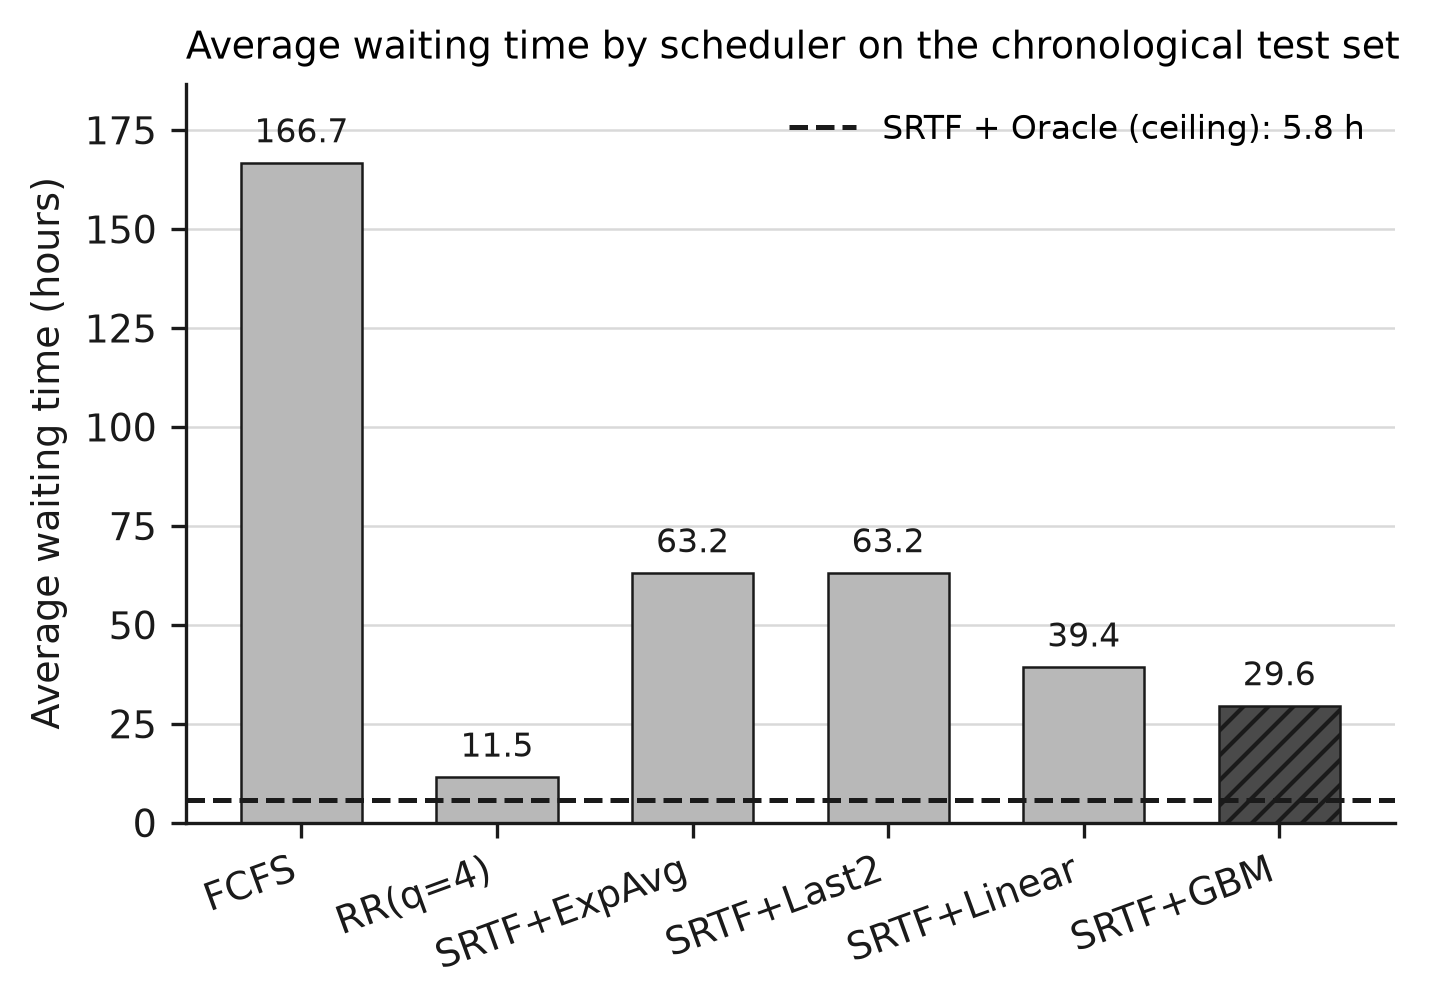
\includegraphics[width=\columnwidth]{../results/figures/fig1_waiting_time_by_scheduler.png}
  \caption{Average waiting time per task by scheduler on the chronological
  test split. The dashed line is the oracle-driven SRTF ceiling.}
  \label{fig:waiting}
\end{figure}

\begin{figure}[t]
  \centering
  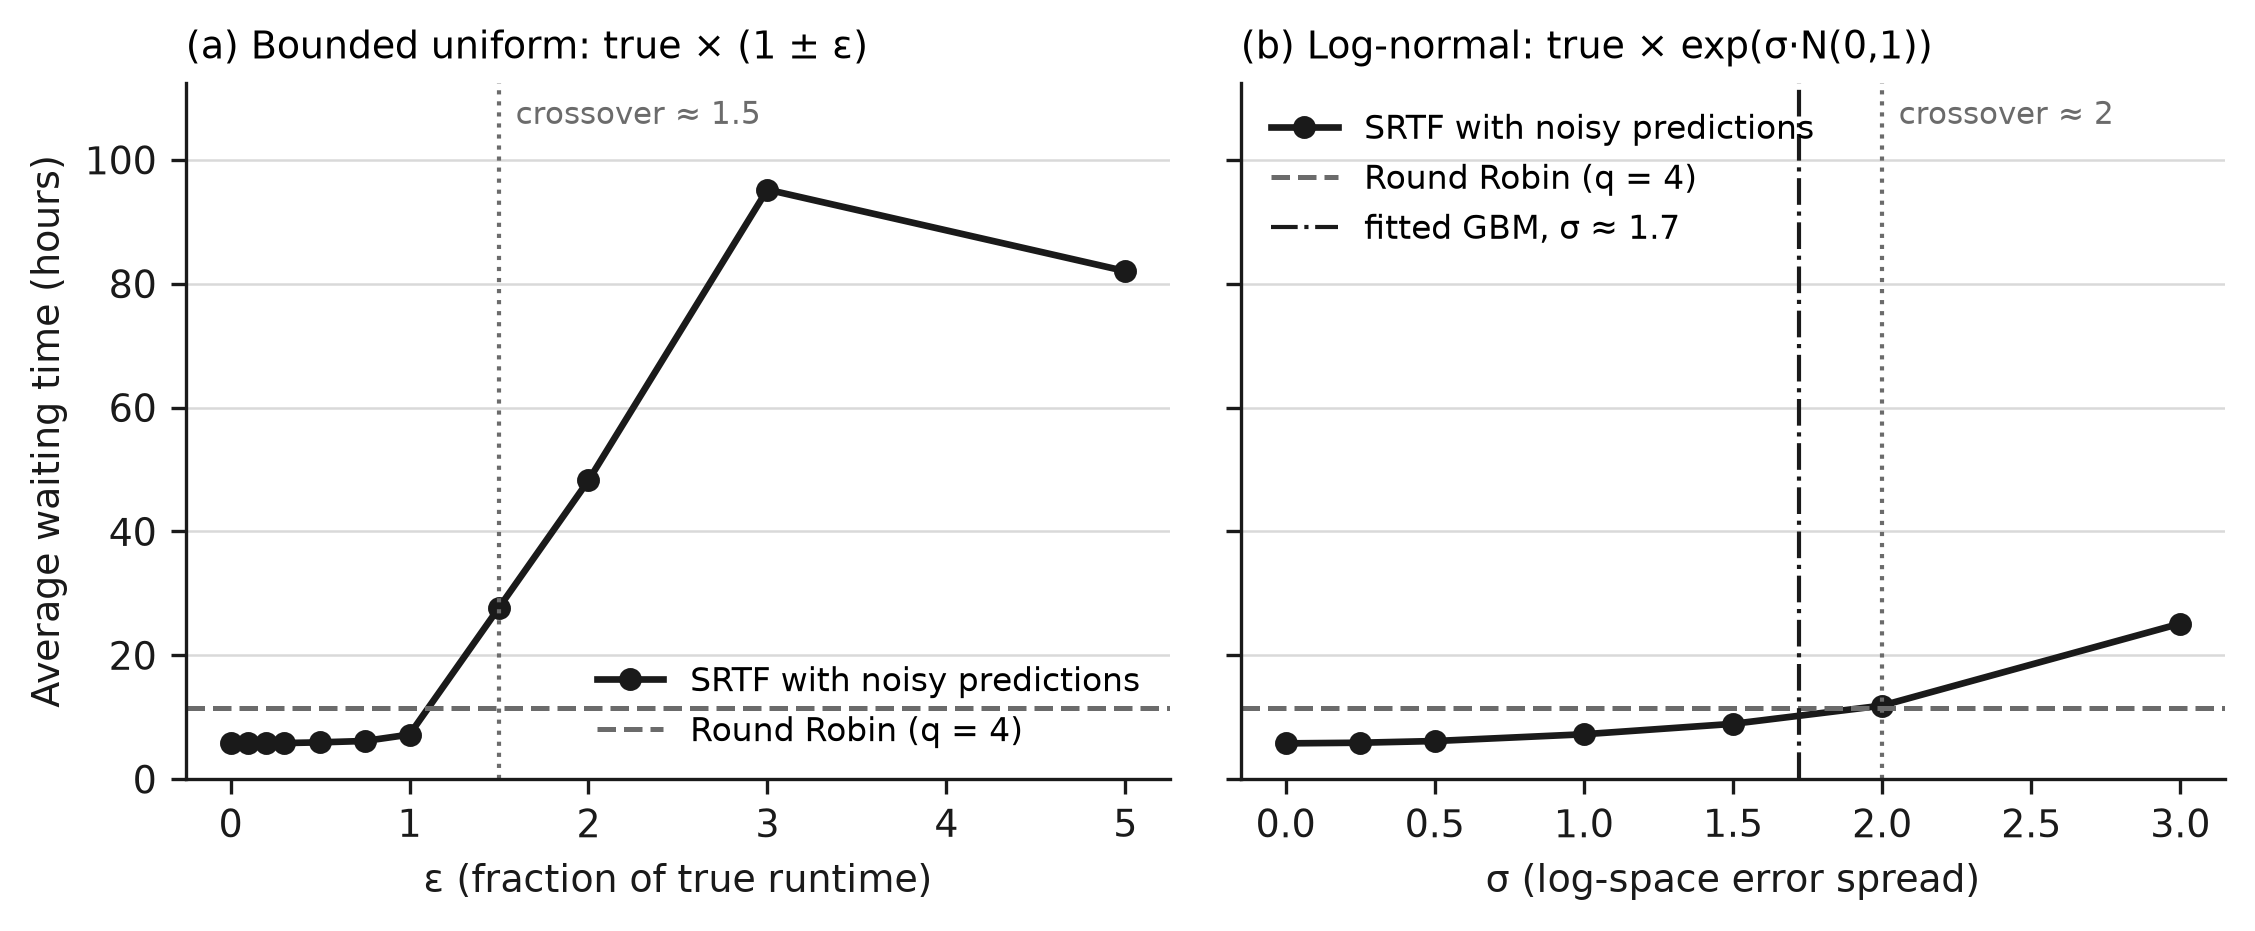
\includegraphics[width=\columnwidth]{../results/figures/fig2_sensitivity.png}
  \caption{Average waiting time of SRTF under injected prediction error:
  (a) bounded uniform, (b) log-normal. The dashed line is round robin; the
  dash-dotted line in (b) marks the empirical log-error spread of the fitted
  gradient-boosted model.}
  \label{fig:sensitivity}
\end{figure}

\begin{figure}[t]
  \centering
  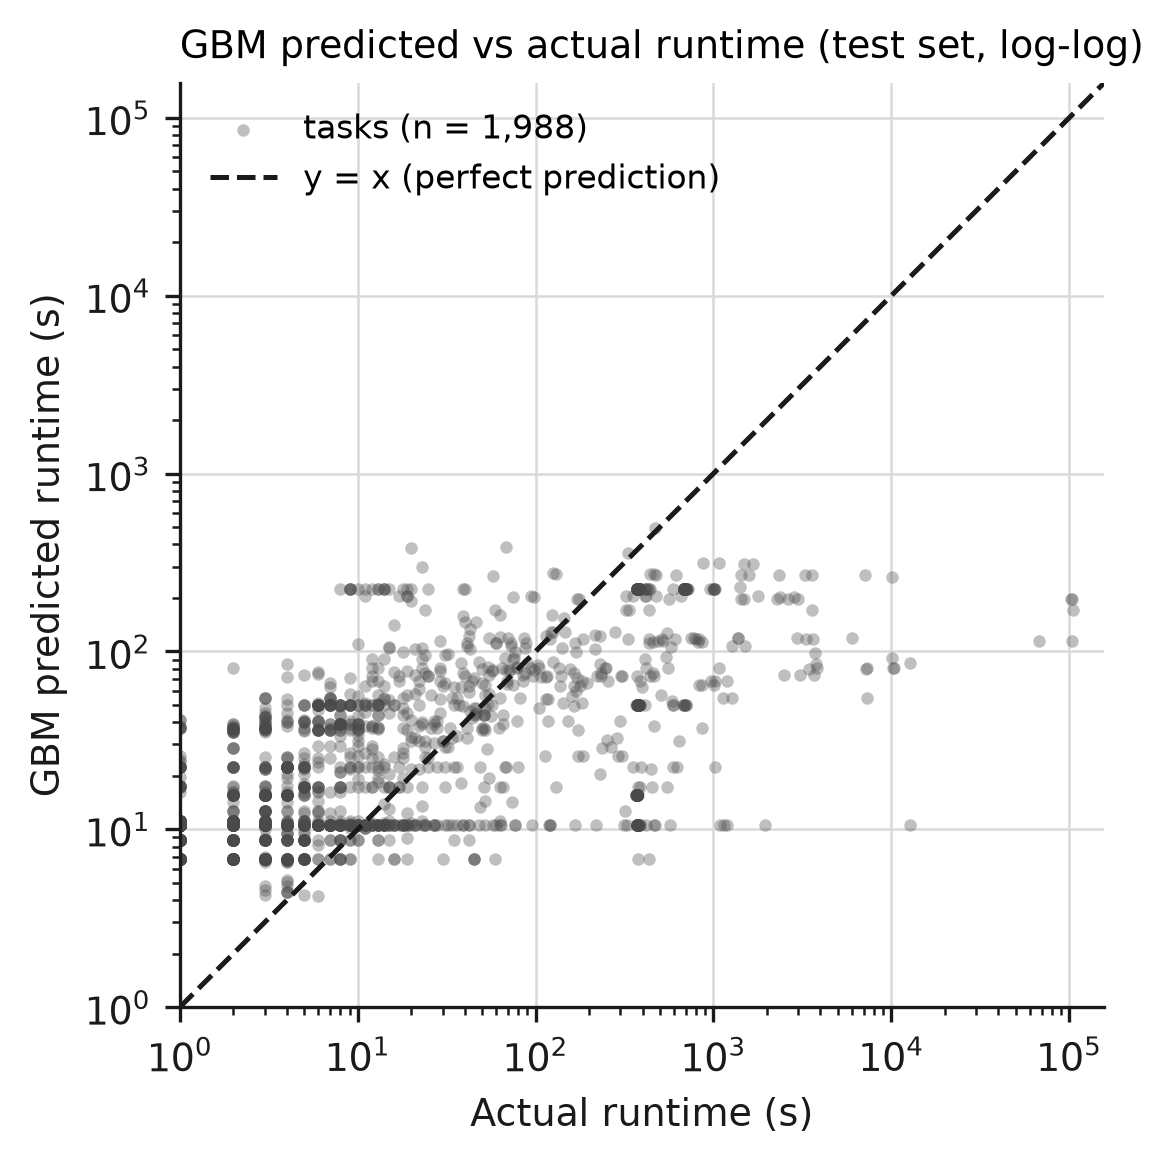
\includegraphics[width=\columnwidth]{../results/figures/fig3_gbm_predicted_vs_actual.png}
  \caption{Gradient-boosted predicted versus actual runtime on the test split
  (log--log). The dashed diagonal is perfect prediction.}
  \label{fig:scatter}
\end{figure}

\section{Threats to Validity}
\label{sec:threats}

\emph{Arrival-time proxy.} The \texttt{batch\_task} table records no
submission time, so arrival is the recorded start time. Any queueing delay
before a task started is invisible, and ``arrival'' here means ``became
runnable''. The causal ordering of historical features and the temporal
features are all defined relative to this proxy.

\emph{Prediction target.} The target is task-level runtime, the duration of
one stage of a job executed by many instances. It is neither a CPU burst
between I/O operations, which (\ref{eq:expavg}) was designed to estimate,
nor strictly a whole job. The simulator treats it as a single CPU demand.

\emph{Short slice and batch-like test set.} The \nTasks{} tasks span about
24 hours, and every test task arrives within \testWindow{}\,s. The
\texttt{hour\_of\_day} and \texttt{day\_of\_week} features therefore act as
indicators of position in the slice rather than of any daily or weekly
cycle, although they are among the gradient-boosted model's most important
features. The near-simultaneous arrivals also mean that preemption plays
almost no role in the test period, so the results characterise batch
ordering more than online preemptive scheduling.

\emph{Single trace, simulation and uncharged inference.} All results come
from one trace and a simulator. Preemption cost is not modelled, the cost of
running a predictor is not charged against scheduling latency, and no
kernel implementation was attempted. The results may not transfer to other
workloads.

\emph{Single noise draws.} Each sensitivity level uses one random draw, so
individual points carry sampling noise, as the non-monotone uniform sweep at
its largest levels shows. The crossover levels should be read as
approximate.

\emph{Weak learned models.} On this slice the learned models barely improve
on a constant median in mean absolute error. The recovery percentage must
therefore be read together with the round-robin comparison, not instead of
it.

\section{Conclusion and Future Work}
\label{sec:conclusion}

This paper measured how much of the waiting-time advantage of clairvoyant
SRTF a learned, arrival-time runtime predictor can recover on a production
cluster trace. A gradient-boosted model recovers \headline{} of the gap
between exponential-averaging SRTF and oracle SRTF, but it does not make
SRTF competitive with round robin, which uses no prediction at all. The
reason is that the information SRTF needs most, which of the arriving tasks
are the rare very long ones, is not present in the arrival-time features of
this trace. Mean absolute error hides this failure, while rank correlation
and the scheduling outcome expose it. The sensitivity analysis shows that
the fitted model's error, being concentrated on long tasks, costs several
times more waiting than random error of the same spread.

The specific percentages are properties of this trace slice and will not
transfer. The methodology should: the recovery metric, the causality tests
for features and online baselines, the oracle-equivalence test for the
simulator, and the contrast between structured and random error apply to
any trace.

Three directions follow directly from the results. First, predictions should
be revised once a task's elapsed service exceeds them, which closes the
failure mode in which an under-predicted long task cannot be preempted.
Second, the evaluation should be repeated on a slice spanning several days
and on a second trace, such as the Google 2019 trace or GWA-T-4, so that
temporal features can capture genuine periodicity and arrivals are spread
out in time. Third, quantile or classification predictors that target the
question ``is this task one of the very long ones?'' address the decision
the scheduler actually makes more directly than mean-error regression does.

\bibliographystyle{IEEEtran}
\bibliography{refs}

\end{document}
